\documentclass[letterpaper, reqno,11pt]{article}
\usepackage[margin=1.0in]{geometry}
\usepackage{color,latexsym,amsmath,amssymb,graphicx,float,listings,tikz}
\usepackage{hyperref}

\hypersetup{
colorlinks=true,
linkcolor=magenta,
filecolor=magenta,
urlcolor=cyan,
}

\graphicspath{ {images/} }

\begin{document}
\pagenumbering{arabic}
\title{Math 406 Homework 2}
\date{10/10/23}
\author{Xander Naumenko}
\maketitle

{\medskip\noindent\bf Question 1.} See tables \ref{tab:q1a}, \ref{tab:q1b}, \ref{tab:q1c}, \ref{tab:q1d} and \ref{tab:q1e} for the required tables. For the log-log plots see figures \ref{fig:q1a}, \ref{fig:q1b}, \ref{fig:q1c}, \ref{fig:q1d} and \ref{fig:q1e}.

The code for this question can be seen here:
\begin{lstlisting}
disp('midpoint')
numerical_integration(-1, 1, @(x) 1/(1+x^2)^0.5, 32, 1);
disp('trap')
numerical_integration(-1, 1, @(x) 1/(1+x^2)^0.5, 32, 2);
disp('simpson')
numerical_integration(-1, 1, @(x) 1/(1+x^2)^0.5, 32, 3);
disp('gauss_legendre')
numerical_integration(-1, 1, @(x) 1/(1+x^2)^0.5, 32, 4);
disp('real')
% -2*log(2^0.5-1)

functions = {@(x) 1/(1+x^2)^0.5, @(x) sin(2*x)^2, @(x) x^(4.0/3), @(x) x^(1.0/3), @(x) (-log(x))^0.5};
bounds = [-1,1; 0,pi; 0,1; 0,2; 0,1];
real_ans = [-2*log(2^0.5-1), pi/2, 3.0/7, 3/(2^(2.0/3)), pi^0.5/2];
Ns = [2,4,16,32];
tables = zeros(5,4,5);
for i = 1:length(functions)
    f = functions{i};
    for j = 1:length(Ns)
        N = Ns(j);
        for choice = [1,2,3,4]
            if i ~= 5 || (choice ~= 2 && choice ~= 3)
                tables(i,j,choice) = numerical_integration(bounds(i,1),bounds(i,2),f,N,choice);
            end
        end
        tables(i,j,5) = real_ans(i);
    end
end

for i = 1:5
    disp(array2table(squeeze(tables(i,:,:))))
end


% Calculate the errors
errors = abs(tables - real_ans');

methods = {'Midpoint', 'Trapezium', 'Simpson', 'Gauss-Legendre'};
colors = {'r', 'g', 'b', 'k'};

for func_idx = 1:5
    figure('Name', ['Function ' num2str(func_idx)]); % Creates a new figure for each function
    hold on;
    for choice = 1:4
        loglog(Ns, squeeze(errors(func_idx, :, choice)), '-o', 'Color', colors{choice}, 'DisplayName', methods{choice});
    end
    xlabel('N');
    ylabel('Error');
    title(['Log-Log plot of N vs Error for Function ', num2str(func_idx)]);
    
    % Ensuring that the axes are in log-log scale
    set(gca, 'XScale', 'log', 'YScale', 'log');
    
    legend('Location', 'southwest');
    grid on;
    hold off;
end

% 1. Midpoint rule with N cells
% 2. Trapezium rule with N cells
% 3. Simpson''s rule with 2N cells
% 4. Three-point Gauss-Legendre quadrature with N cells
function result = numerical_integration(a, b, f, N, choice)

    switch choice
        case 1
            result = midpoint_rule(f, a, b, N);
        case 2
            result = trapezium_rule(f, a, b, N);
        case 3
            result = simpsons_rule(f, a, b, N);
        case 4
            result = gauss_legendre(f, a, b, N);
        otherwise
            return;
    end

    % fprintf('The result of the integration is: %.5f\n', result);
end

function result = midpoint_rule(f, a, b, N)
    result = 0;
    for i = 0:(N-1)
        point = a+(i+0.5)*(b-a)/N;
        result = result + f(point);
    end

    result = result * (b-a)/N;
end


function result = trapezium_rule(f, a, b, N)
    result = 0;
    for i = 1:(N-1)
        point = a+i*(b-a)/N;
        result = result + 2*f(point);
    end
    result = result + f(a) + f(b);

    result = result * (b-a)/N/2;
end

function result = simpsons_rule(f, a, b, N)
    result = 0;
    for i = 1:N
        left = a+(i-1)*(b-a)/N;
        right = a+i*(b-a)/N;
        result = result + 1/3*(b-a)/N/2*(f(left)+4*f((left+right)/2)+f(right));
    end
end

function result = gauss_legendre(f, a, b, N)
    x = [-sqrt(3/5), 0, sqrt(3/5)];
    w = [5/9, 8/9, 5/9];

    result = 0;
    for i = 1:N
        left = a + (i-1)*(b-a) / N;
        right = a + i*(b-a)/N;
        for j = 1:3
            xi = 0.5*(left+right + (right-left) * x(j));
            result = result+w(j)*f(xi);
        end
    end
    result = 0.5 * (b-a)/N*result;
end
\end{lstlisting}

\begin{table}
\centering
\begin{tabular}{|c|c|c|c|c|}
\hline
$N$ & Midpoint & Trapezium & Simpson & Gauss-Legendre \\
\hline
2 & 1.78885438199983 & 1.70710678118655 & 1.76160518172874 & 1.76266240387583 \\
\hline
4 & 1.77014250014533 & 1.74798058159319 & 1.76275519396128 & 1.76274697462844 \\
\hline
16 & 1.76320768598367 & 1.7618262836833 & 1.76274721855022 & 1.76274717401768 \\
\hline
32 & 1.76286227284615 & 1.76251698483349 & 1.76274717684193 & 1.76274717403875 \\
\hline
\end{tabular}
\caption{Question 1a}
\label{tab:q1a}
\end{table}

\begin{table}
\centering
\begin{tabular}{|c|c|c|c|c|}
\hline
$N$ & Midpoint & Trapezium & Simpson & Gauss-Legendre \\
\hline
2 & 3.14159265358979 & 7.06745147303987e-32 & 2.0943951023932 & 1.60606730241802 \\
\hline
4 & 1.5707963267949 & 1.5707963267949 & 1.5707963267949 & 1.5707963267949 \\
\hline
16 & 1.5707963267949 & 1.5707963267949 & 1.5707963267949 & 1.5707963267949 \\
\hline
32 & 1.5707963267949 & 1.5707963267949 & 1.5707963267949 & 1.5707963267949 \\
\hline
\end{tabular}
\caption{Question 1b}
\label{tab:q1b}
\end{table}

\begin{table}
\centering
\begin{tabular}{|c|c|c|c|c|}
\hline
$N$ & Midpoint & Trapezium & Simpson & Gauss-Legendre \\
\hline
2 & 0.419455176774456 & 0.448425131496025 & 0.429111828348312 & 0.428525592513674 \\
\hline
4 & 0.426049167558007 & 0.43394015413524 & 0.428679496417085 & 0.428562331914328 \\
\hline
16 & 0.428391866554757 & 0.428943359698886 & 0.4285756976028 & 0.428571070406974 \\
\hline
32 & 0.428524607238247 & 0.428667613126822 & 0.428572275867772 & 0.428571357502592 \\
\hline
\end{tabular}
\caption{Question 1c}
\label{tab:q1c}
\end{table}

\begin{table}
\centering
\begin{tabular}{|c|c|c|c|c|}
\hline
$N$ & Midpoint & Trapezium & Simpson & Gauss-Legendre \\
\hline
2 & 1.93841476853743 & 1.62996052494744 & 1.83559668734077 & 1.89373800719319 \\
\hline
4 & 1.91040464923353 & 1.78418764674243 & 1.86833231506983 & 1.89141202322811 \\
\hline
16 & 1.89332086475362 & 1.8728210349583 & 1.88648758815518 & 1.89012260552418 \\
\hline
32 & 1.89126652809474 & 1.88307094985596 & 1.88853466868182 & 1.8899772279319 \\
\hline
\end{tabular}
\caption{Question 1d}
\label{tab:q1d}
\end{table}

\begin{table}
\centering
\begin{tabular}{|c|c|c|c|c|}
\hline
$N$ & Midpoint & Trapezium & Simpson & Gauss-Legendre \\
\hline
2 & 0.856885021909063 & 0 & 0 & 0.881394330687781 \\
\hline
4 & 0.870845677383917 & 0 & 0 & 0.883847456341008 \\
\hline
16 & 0.882289474604227 & 0 & 0 & 0.885658742625317 \\
\hline
32 & 0.884274758802113 & 0 & 0 & 0.88595040876536 \\
\hline
\end{tabular}
\caption{Question 1e}
\label{tab:q1e}
\end{table}

\begin{figure}[htpb]
    \centering
    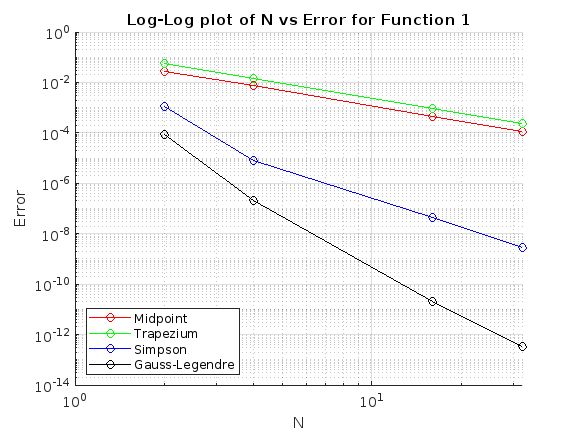
\includegraphics[width=0.8\textwidth]{q1a}
    \caption{Error of Question 1a.}
    \label{fig:q1a}
\end{figure}
\begin{figure}[htpb]
    \centering
    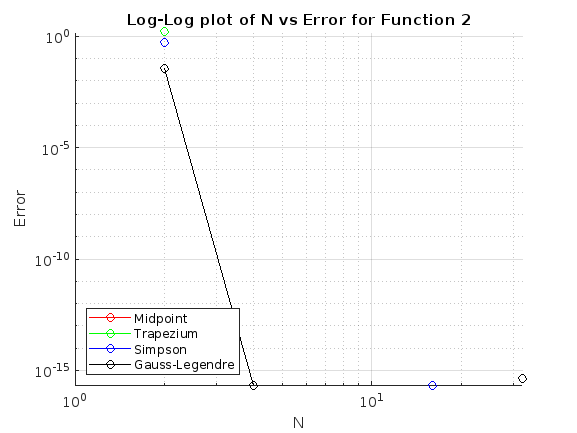
\includegraphics[width=0.8\textwidth]{q1b}
    \caption{Error of Question 1b. Note that due to the fact that the error goes to zero very quickly for the different methods by chance means this plot doesn't look like the others.}
    \label{fig:q1b}
\end{figure}
\begin{figure}[htpb]
    \centering
    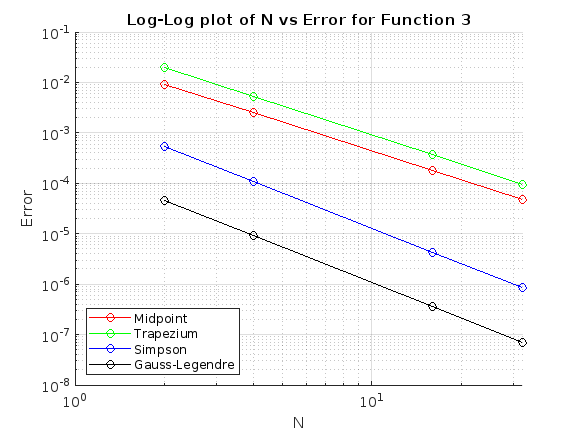
\includegraphics[width=0.8\textwidth]{q1c}
    \caption{Error of Question 1c.}
    \label{fig:q1c}
\end{figure}
\begin{figure}[htpb]
    \centering
    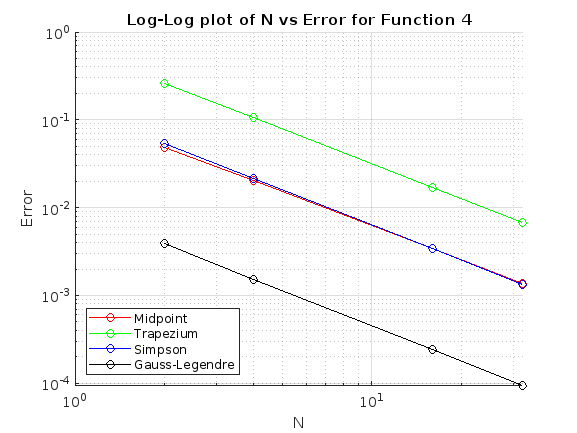
\includegraphics[width=0.8\textwidth]{q1d}
    \caption{Error of Question 1d.}
    \label{fig:q1d}
\end{figure}
\begin{figure}[htpb]
    \centering
    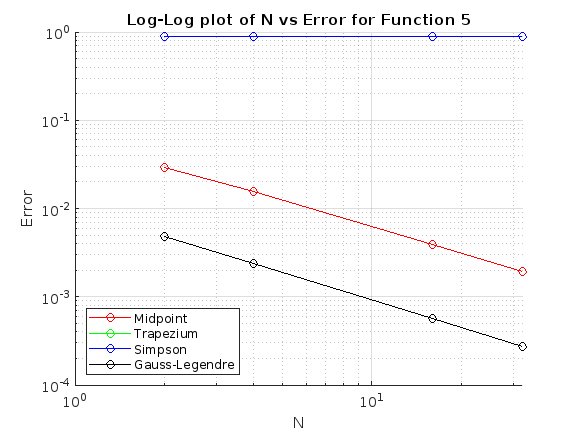
\includegraphics[width=0.8\textwidth]{q1e}
    \caption{Error of Question 1e. Ignore the error for trapezium/Simpson, they were set to 0 in the code so had a constant error.}
    \label{fig:q1e}
\end{figure}

{\medskip\noindent\bf Question 2.} Using the given asymptotic expansion for the Trapezium rule error, we get
\[
I(0)-I(h_{s+1})=I(0)-I(\frac{1}{2}h_s)=\sum_{i=1}^{\infty}\frac{1}{2^{2i}}c_ih_s^{2i}
\]
\[
\implies 4I(\frac{1}{2}h_s)=4I(0)-\sum_{i=1}^{\infty}\frac{1}{2^{2i}}c_ih_s^{2i}
\]
\[
\implies I(0)=\frac{4I(\frac{h_2}{2})-I(h_2)}{3}+ \sum_{i=2}^{\infty}\frac{2^{2i}-1}{3\cdot 2^{2i}}c_i h_s^{2i}
.\]
Define $a_s^{(1)}=I(h_s)$ and $c_i^{(2)}$ as in the question. Then simply rearranging the above formula algebraically, we get
\[
I(0)-\left(I(\frac{h_2}{2})+\frac{I(\frac{h_2}{2})-I(h_s)}{3}\right)=I(0)-a_{s+1}^{(1)}-\frac{a_{s+1}^{(1)}-a_s^{(1)}}{3}=\sum_{i=2}^{\infty}c_{i}^{(2)}h_s^{2i}
.\]


\end{document}
